\documentclass[12pt]{extarticle}
\usepackage[utf8]{inputenc}
\usepackage{graphicx}
\usepackage{float}

% Disable indentation
\setlength{\parindent}{0pt}

\title{Lab 9: PKI HTTPS PROXY}
\author{Alexander Hoffmann \and Sofiane Rahli \and Yvan Compaore}
\date{\today}

\begin{document}

\maketitle

\section{Network configuration}
\textbf{1.} As we start the PC Router virtual machine, we need to modify the IP configuration. First, enable the interface connected to the internet. To show all the available interfaces, use:
\begin{verbatim}
ip link
\end{verbatim}
\begin{center}
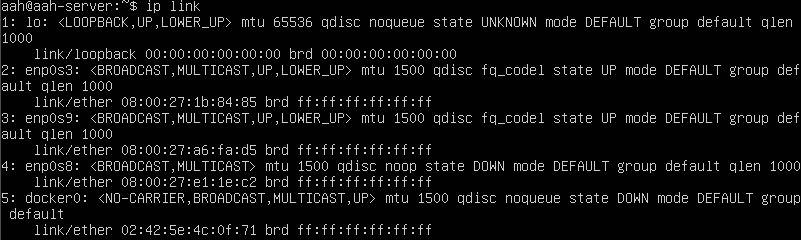
\includegraphics[scale=0.45]{resources/1-1-1.png}\\
\end{center}
There are 3 ip interfaces that interest us. \texttt{enp0s3} and \texttt{enp0s9} are host-only adapters. Observe that interface \texttt{enp0s8} is down. It corresponds to the NAT interface in the VirtualBox network configuration. We need to enable the interface and assign it an IP address using DHCP.
\begin{verbatim}
ifconfig enp0s8 up
\end{verbatim}
Now the interface is enabled but it does not have an IP address. To ask for a new DHCP lease, use:
\begin{verbatim}
dhclient enp0s8
\end{verbatim}
Now the DHCP sent a lease and the interface now has an IP address and an active internet connection.
\begin{center}
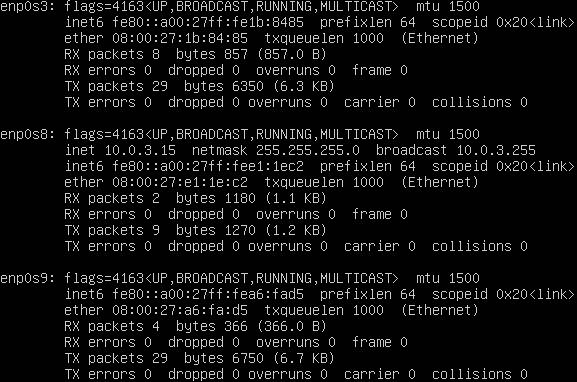
\includegraphics[scale=0.6]{resources/1-1-2.png}\\
\end{center}
To prove that the VM is connected to the internet, we ping the \texttt{google.com} server.
\begin{center}
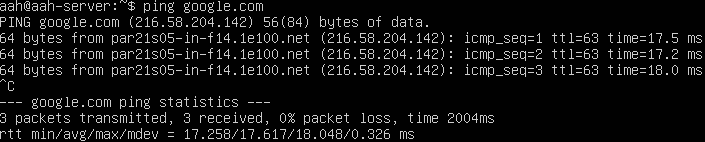
\includegraphics[scale=0.5]{resources/1-1-3.png}\\
\end{center}

\textbf{2.} 

\end{document}
